\documentclass[12pt, b5paper]{article}
\usepackage{ctex}

\usepackage{geometry}
\geometry{b5paper,left=2cm,right=1cm,top=2.5cm,bottom=2.5cm}
\usepackage{chemformula} %化学公式宏包
\usepackage[version=4]{mhchem} %化学公式宏包
\usepackage{siunitx} %数字，单位宏包
\sisetup{
	separate-uncertainty = true,
	inter-unit-product = \ensuremath{{}\cdot{}}
} %单位间加小圆点
\usepackage{tikz} %Tikz绘图包
\usetikzlibrary{cd}
\usetikzlibrary{chains}
\usetikzlibrary{arrows}
\usetikzlibrary{arrows.meta} %画箭头
\usetikzlibrary{commutative-diagrams} %交换图
\usetikzlibrary{positioning,automata}
\usepackage[all]{xy}
\usepackage{booktabs} %三线表
\usepackage{multirow} %合并单元格
\usepackage{makecell} %表格内强制换行
\usepackage{array}
\usepackage{booktabs} %控制表格行高
\usepackage{colortbl}  %彩色表格需要加载的宏包
\usepackage{amsmath}
\usepackage{unicode-math}
\usepackage{fontspec} %字体
\newcommand*{\cred}{\textcolor{red}}

\setmainfont{Times New Roman}
\setmathfont{XITS Math}

\setlength{\parindent}{0pt} %无缩进
\usepackage{setspace}
\usepackage{fancyhdr} %设置页码
\usepackage{lastpage} %获取总页数
\pagestyle{fancy} %fancyhdr宏包新增的页面风格
\renewcommand\headrulewidth{0pt} %取消页眉中的装饰分割线
\fancyhf{}
\cfoot{\footnotesize 第 \thepage\ 页(共 \pageref{LastPage}页)}%当前页 of 总页数


%微分符号
\makeatletter
\newcommand*{\dif}{\mathop{}\!\mathrm{d}}
\makeatother

%直立积分
\DeclareSymbolFont{EulerExtension}{U}{euex}{m}{n}
\DeclareMathSymbol{\euintop}{\mathop} {EulerExtension}{"52}
\DeclareMathSymbol{\euointop}{\mathop} {EulerExtension}{"48}
\let\intop\euintop
\let\ointop\euointop



\begin{document}
\begin{spacing}{1.625}

\centerline{{\huge 河北农业大学课程考试试卷}}

\centerline{\large 2023-2024学年第\underline{\ 1\ }学期}

考试科目：\underline{化学反应工程} \hfill 姓名：\underline{ \qquad \qquad} \hfill 学号：\underline{ \qquad \qquad \qquad \qquad}

学院：\underline{理工学院} \hfill 专业班级：\underline{\qquad \qquad \qquad \qquad} \hfill 卷别：\cred{A} \hfill 考核方式：\cred{开卷}

（注：考生务必将答案写在答题纸上，标清楚大小题号，写在本试卷上无效）

\bigskip

{\bfseries 一、简答题（共40分）}

1. (8分) 以纯A为原料在连续釜式反应器中生产产物P，P的收率与温度的关系如下图所示。你认为反应在什么温度下进行比较合适？说明理由。
\begin{figure}[htpb]
	\centering
	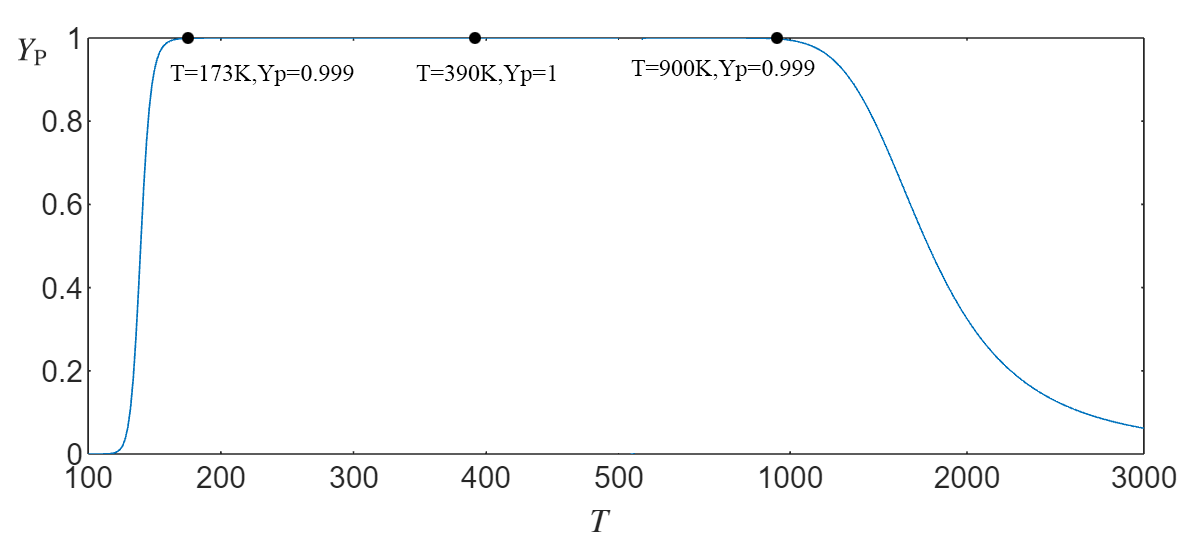
\includegraphics[width=\linewidth]{images/Yp}
\end{figure}

2. (12分) 概述反应器设计的基本内容，反应器设计基本方程。

\bigskip
\bigskip

3. (9分) 非理想流动模型有哪几种？各模型的模型参数分别是？

\bigskip
\bigskip

4. (11分) 试列出气固相催化反应通常所经历的步骤，并区分哪些步骤为动力学控制，哪些步骤为传递控制。

\newpage
{\bfseries 二、计算题（共60分）}

1. (20分) 某液相均相反应：
\vspace{-1.5em}
\[
	\ch{A + B -> P} \qquad r = kc_\mathrm{A}c_\mathrm{B}
	\vspace{-1.5em}
\]
当反应温度100℃时，反应速率常数为\SI{0.5}{L.mol^{-1}.h^{-1}}，进料混合物中A、B的初始浓度均为2 mol/L。要求P的产量为80 mol/h，最终转化率为80\%。求下列几种情况下的反应体积：

（1）反应在间歇釜式反应器中进行，辅助时间为1 h；

（2）反应在全混流釜式反应器中进行；

（3）反应在活塞流管式反应器中进行。

\bigskip
\bigskip

2. (20分) 现有一台\SI{2}{m^3}的全混流反应器，进行液相一级不可逆反应： 
\vspace{-1.5em}
\[
	\ch{A -> 2 R} \qquad r = kc_\mathrm{A}
	\vspace{-1.5em}
\]
当处理量$Q_0=1\ \mathrm{m^3/h}$时，出口转化率达80\%。现在原反应器后串联一只反应器，反应温度相同。若处理量增加一倍，则：

（1）串联一只全混流反应器，总出口转化率仍为80\%，该反应体积为多大？

（2）若串联一只\SI{2}{m^3}的全混流反应器，总出口转化率可达多少？


\bigskip
\bigskip

3. (20分) 在直径8 mm的球形催化剂上进行丁烷脱氢反应，其反应速率方程为
\vspace{-1.5em}
\[
	r_{\mathrm{A}} =k_{\mathrm{W}} c_{\mathrm{A}} \quad \mathrm{mol} /(\mathrm{g} \cdot \mathrm{s})
	\vspace{-1.5em}
\]
0.1013 MPa及773 K时，$k_\mathrm{W} = \SI{0.92}{cm^3/(g.s)}$。若催化剂平均孔半径为\SI{4e-7}{cm}，孔容为\SI{0.35}{cm^3/g}，曲节因子等于2.5。试计算内扩散有效因子。

（注：$\tanh (x) = \frac{\mathrm{e}^x - \mathrm{e}^{-x}}{\mathrm{e}^x + \mathrm{e}^{-x}}$。当$x>3$时，$\tanh (x) = 1$）


\end{spacing}
\end{document}
